154. \begin{figure}[ht!]
\center{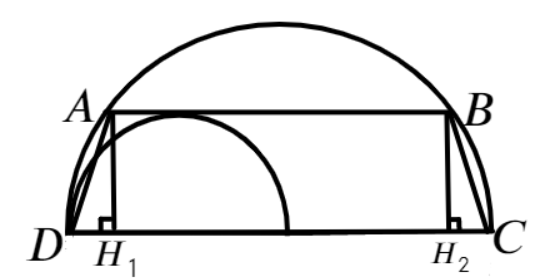
\includegraphics[scale=0.35]{g9-154.png}}
\end{figure}\\
Рассмотрим трапецию $ABCD:$ она вписанная и поэтому равнобедренная, её основания равны 12 и $2R,$ а высота --- $r,$ где $R$ и $r$ являются радиусами большей и меньшей полуокружности соответственно. Опустим высоты $AH_1$ и $BH_2,$ тогда $DH_1=H_2C=\cfrac{2R-12}{2}=R-6.$ Угол $DAC$ опирается а диаметр, значит он прямой и треугольник $DAC$ прямоугольный, тогда по теореме Пифагора $AC^2=4R^2-AD^2.$ С другой стороны, из треугольника $ACH_1$ имеем $AC^2=r^2+(12+R-6)^2=r^2+(R+6)^2,$ а из треугольника $ADH_1$ --- $AD^2=(R-6)^2+r^2.$ Значит, $4R^2-(R-6)^2-r^2=r^2+(R+6)^2,\ 4R^2-R^2+12R-36=2r^2+R^2+12R+36,$ откуда $R^2-r^2=36.$ Искомая площадь равна $\cfrac{\pi R^2}{2}-\cfrac{\pi r^2}{2}=\cfrac{\pi(R^2-r^2)}{2}=\cfrac{\pi\cdot36}{2}=18\pi.$\newpage\noindent
